\pagebreak

\subsection{Приложение}

\subsubsection{Эксперимент 1}
\begin{figure}[h!]
    \centering
    \includegraphics[width=0.8\textwidth]{assets/1/fixed.png}
    % \caption{Фиксированный $a_n$. $lambda =0.01$ }
    \label{exp1:fixed}
\end{figure}
\begin{figure}[h!]
    \centering
    \includegraphics[width=0.8\textwidth]{assets/1/lambda_0.1.png}
    % \caption{Классический Роббинса-Монро.$lambda =0.1$ }
    \label{exp1:lambda_0.1}
\end{figure}
\begin{figure}[h!]
    \centering
    \includegraphics[width=0.8\textwidth]{assets/1/lambda_0.5.png}
    % \caption{Классический Роббинса-Монро.$lambda =0.5$ }
    \label{exp1:lambda_0.5}
\end{figure}
\begin{figure}[h!]
    \centering
    \includegraphics[width=0.8\textwidth]{assets/1/adaptive.png}
    % \caption{Предложенный алгоритм}
    \label{exp1:adaptive}
\end{figure}
\pagebreak
\subsubsection{Эксперимент 2}
\begin{figure}[h!]
    \centering
    \includegraphics[width=0.8\textwidth]{assets/2/fixed.png}
    % \caption{Фиксированный $a_n$. $lambda =0.01$ }
    \label{exp2:fixed}
\end{figure}
\begin{figure}[h!]
    \centering
    \includegraphics[width=0.8\textwidth]{assets/2/lambda_0.1.png}
    % \caption{Классический Роббинса-Монро.$lambda =0.1$ }
    \label{exp2:lambda_0.1}
\end{figure}
\begin{figure}[h!]
    \centering
    \includegraphics[width=0.8\textwidth]{assets/2/lambda_0.5.png}
    % \caption{Классический Роббинса-Монро.$lambda =0.5$ }
    \label{exp2:lambda_0.5}
\end{figure}
\begin{figure}[h!]
    \centering
    \includegraphics[width=0.8\textwidth]{assets/2/adaptive.png}
    % \caption{Предложенный алгоритм}
    \label{exp2:adaptive}
\end{figure}
\pagebreak
\subsubsection{Эксперимент 3}
\begin{figure}[h!]
    \centering
    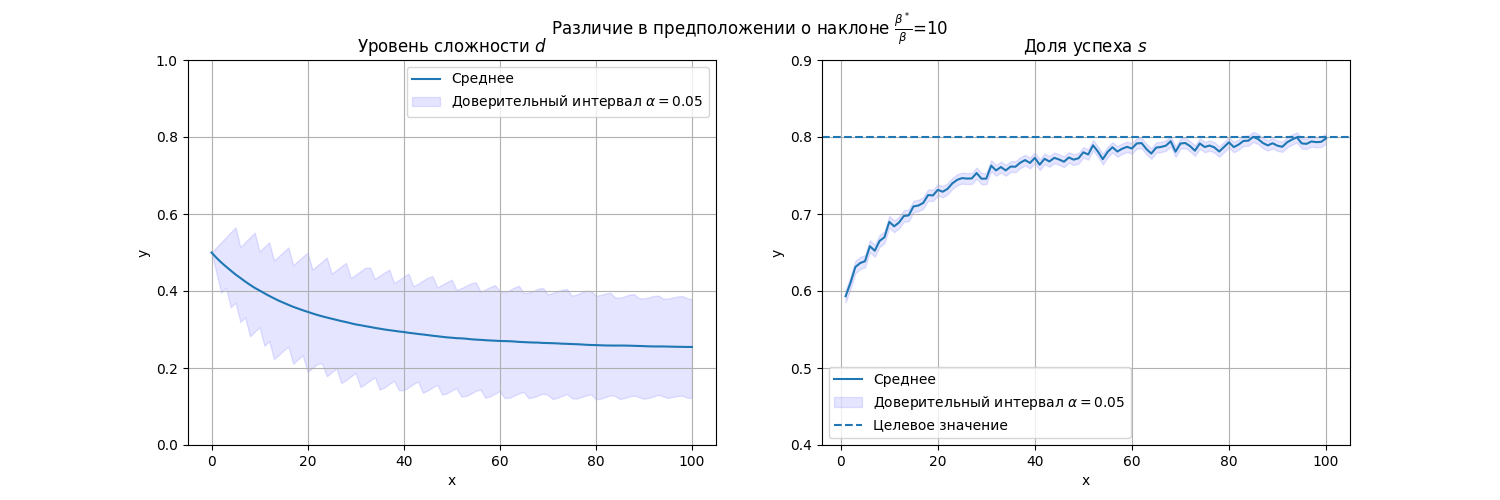
\includegraphics[width=0.8\textwidth]{assets/3/0.png}
     % \caption{Предложенный алгоритм}
    \label{exp3:10}
\end{figure}
\begin{figure}[h!]
    \centering
    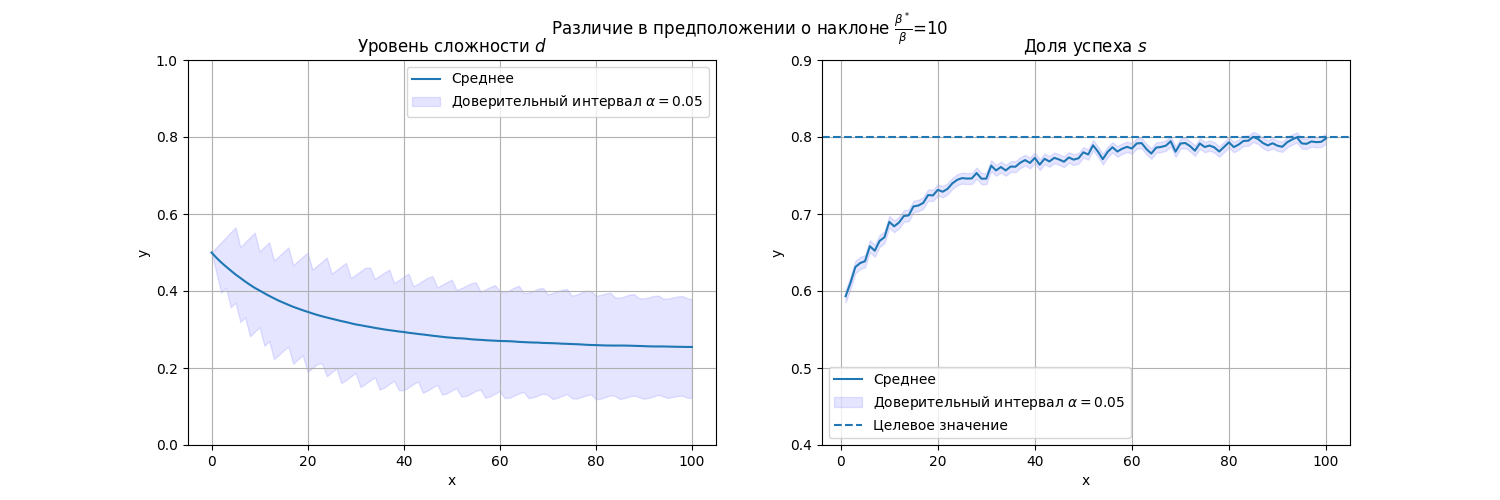
\includegraphics[width=0.8\textwidth]{assets/3/0.png}
    \label{exp3:2_5}
\end{figure}
\begin{figure}[h!]
    \centering
    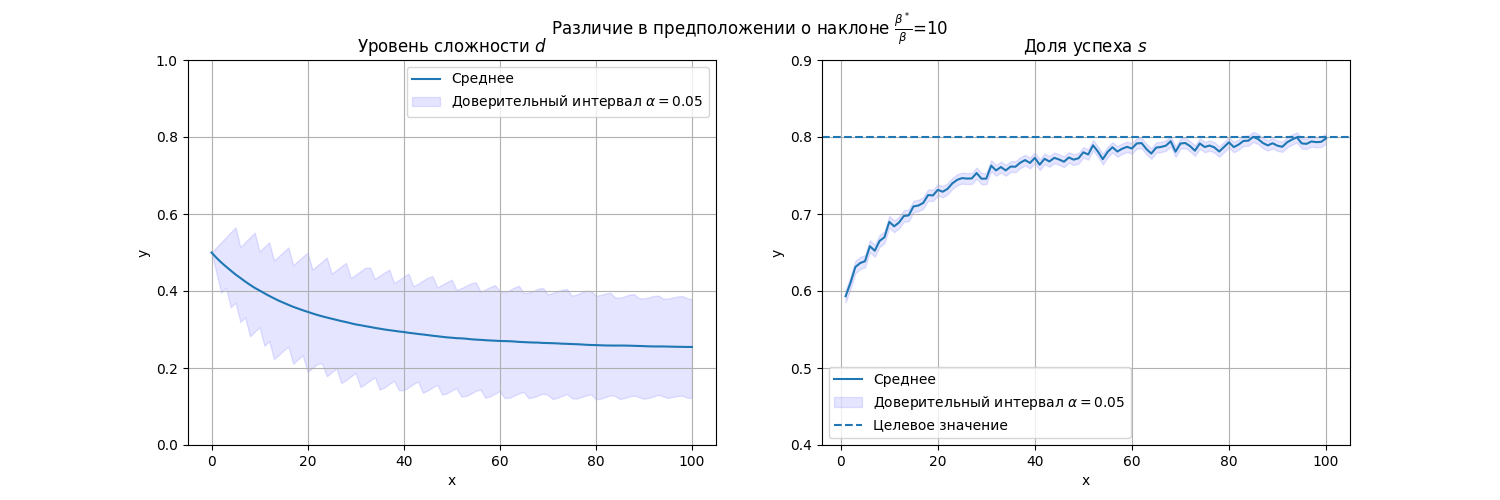
\includegraphics[width=0.8\textwidth]{assets/3/0.png}
    \label{exp3:1}
\end{figure}
\begin{figure}[h!]
    \centering
    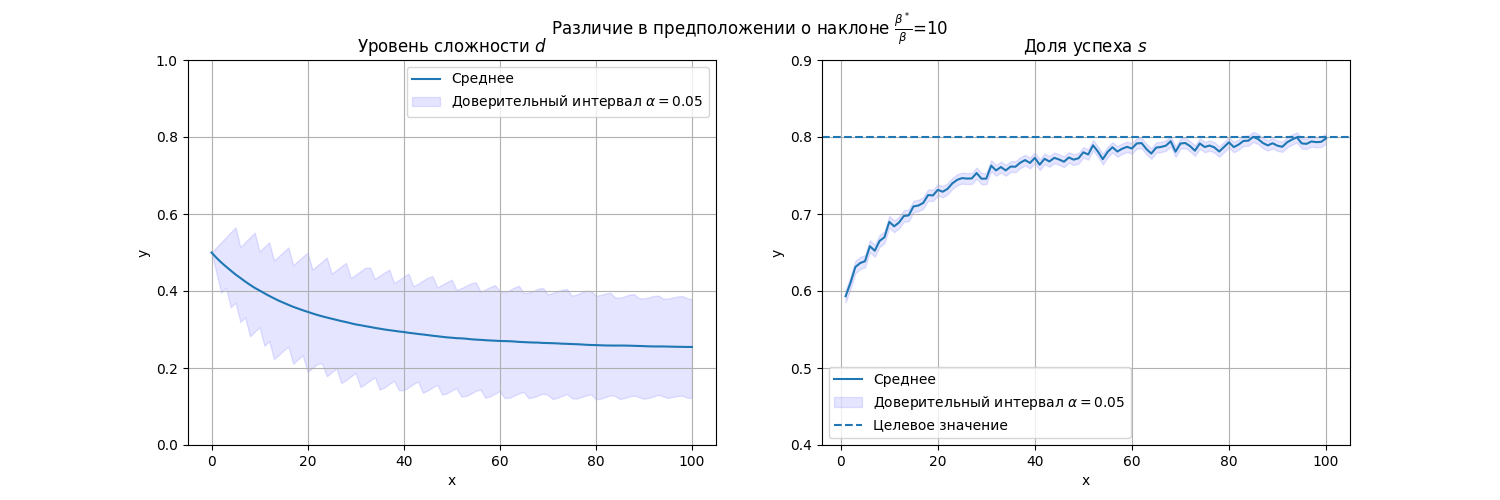
\includegraphics[width=0.8\textwidth]{assets/3/0.png}
    \label{exp3:_0.25}
\end{figure}
\pagebreak
\subsubsection{Эксперимент 4}
\begin{figure}[h!]
    \centering
    \includegraphics[width=0.8\textwidth]{assets/4/adaptive.png}
    % \caption{Предложенный алгоритм}
    \label{exp4:algo}
\end{figure}
\end{document}